\documentclass{beamer}\usepackage[]{graphicx}\usepackage[]{color}
%% maxwidth is the original width if it is less than linewidth
%% otherwise use linewidth (to make sure the graphics do not exceed the margin)
\makeatletter
\def\maxwidth{ %
  \ifdim\Gin@nat@width>\linewidth
    \linewidth
  \else
    \Gin@nat@width
  \fi
}
\makeatother

\definecolor{fgcolor}{rgb}{0.196, 0.196, 0.196}
\newcommand{\hlnum}[1]{\textcolor[rgb]{0.063,0.58,0.627}{#1}}%
\newcommand{\hlstr}[1]{\textcolor[rgb]{0.063,0.58,0.627}{#1}}%
\newcommand{\hlcom}[1]{\textcolor[rgb]{0.588,0.588,0.588}{#1}}%
\newcommand{\hlopt}[1]{\textcolor[rgb]{0.196,0.196,0.196}{#1}}%
\newcommand{\hlstd}[1]{\textcolor[rgb]{0.196,0.196,0.196}{#1}}%
\newcommand{\hlkwa}[1]{\textcolor[rgb]{0.231,0.416,0.784}{#1}}%
\newcommand{\hlkwb}[1]{\textcolor[rgb]{0.627,0,0.314}{#1}}%
\newcommand{\hlkwc}[1]{\textcolor[rgb]{0,0.631,0.314}{#1}}%
\newcommand{\hlkwd}[1]{\textcolor[rgb]{0.78,0.227,0.412}{#1}}%
\let\hlipl\hlkwb

\usepackage{framed}
\makeatletter
\newenvironment{kframe}{%
 \def\at@end@of@kframe{}%
 \ifinner\ifhmode%
  \def\at@end@of@kframe{\end{minipage}}%
  \begin{minipage}{\columnwidth}%
 \fi\fi%
 \def\FrameCommand##1{\hskip\@totalleftmargin \hskip-\fboxsep
 \colorbox{shadecolor}{##1}\hskip-\fboxsep
     % There is no \\@totalrightmargin, so:
     \hskip-\linewidth \hskip-\@totalleftmargin \hskip\columnwidth}%
 \MakeFramed {\advance\hsize-\width
   \@totalleftmargin\z@ \linewidth\hsize
   \@setminipage}}%
 {\par\unskip\endMakeFramed%
 \at@end@of@kframe}
\makeatother

\definecolor{shadecolor}{rgb}{.97, .97, .97}
\definecolor{messagecolor}{rgb}{0, 0, 0}
\definecolor{warningcolor}{rgb}{1, 0, 1}
\definecolor{errorcolor}{rgb}{1, 0, 0}
\newenvironment{knitrout}{}{} % an empty environment to be redefined in TeX

\usepackage{alltt}

% load packages
\usepackage{tikz}
\usepackage{graphicx}
\usepackage{upquote}
\usepackage{listings}
\usepackage{hyperref}
\usepackage{color}
\usepackage{lmodern}



% define a bunch of colors
\definecolor{gray}{RGB}{110,110,110}
\definecolor{darkgray}{RGB}{100,100,100}
\definecolor{lightgray}{RGB}{200,200,200}
\definecolor{lightgrey}{RGB}{200,200,200}
\definecolor{turquoise}{RGB}{81,193,188}
\definecolor{mamey}{RGB}{255,107,107}
\definecolor{tomato}{RGB}{255,136,136}
\definecolor{mandarina}{RGB}{229,169,25}
\definecolor{lemon}{rgb}{0.81,0.95,0.29}
\definecolor{bluesky}{rgb}{0.71,0.81,0.96}
\definecolor{chiclamino}{RGB}{107,174,214}
\definecolor{violet}{RGB}{133,135,211}

\definecolor{foreground}{RGB}{81,141,193}
\definecolor{background}{RGB}{246,244,240}
\definecolor{highlight}{RGB}{229,169,25}
\definecolor{lowlight}{RGB}{200,200,200}

% setting beamer colors
\setbeamercolor{title}{fg=lightgray}
\setbeamercolor{frametitle}{fg=lightgray}
\setbeamercolor{block title}{fg=turquoise}
\setbeamercolor{structure}{fg=turquoise}
\setbeamercolor{titlelike}{fg=title}
\setbeamercolor{subtitle}{fg=turquoise}
\setbeamercolor{institute}{fg=gray}
\setbeamercolor{normal text}{fg=gray,bg=background}

\setbeamercolor{palette primary}{fg=lightgray}
\setbeamercolor{palette secondary}{fg=lightgray}
\setbeamercolor{palette tertiary}{fg=lightgray}

\setbeamerfont{itemize/enumerate subbody}{size=\footnotesize}
\setbeamerfont{itemize/enumerate subitem}{size=\footnotesize}

\hypersetup{
  colorlinks=true,
  urlcolor=tomato,
  linkcolor=lightgray
}

% commands
\newcommand{\code}[1]{\texttt{#1}}
\newcommand{\high}[1]{\textcolor{highlight}{#1}}
\newcommand{\low}[1]{\textcolor{lowlight}{#1}}
\newcommand{\highcode}[1]{\textcolor{highlight}{\texttt{#1}}}


%\usecolortheme{rose}
\setbeamertemplate{blocks}[rounded]
\setbeamertemplate{footline}[frame number] 
\setbeamertemplate{navigation symbols}{}
\setbeamertemplate{frametitle}[default][center]
\useoutertheme{infolines}  % add footlines
\setbeamersize{text margin left=25pt,text margin right=25pt}



% to remove empty brackets of \institution
\makeatletter
\setbeamertemplate{footline}
{
  \leavevmode%
  \hbox{%
  \begin{beamercolorbox}[wd=.333333\paperwidth,ht=2.25ex,dp=1ex,center]{author in head/foot}%
    \usebeamerfont{author in head/foot}\insertshortauthor%~~\beamer@ifempty{\insertshortinstitute}{}{(\insertshortinstitute)}
  \end{beamercolorbox}%
  \begin{beamercolorbox}[wd=.333333\paperwidth,ht=2.25ex,dp=1ex,center]{title in head/foot}%
    \usebeamerfont{title in head/foot}\insertshorttitle
  \end{beamercolorbox}%
  \begin{beamercolorbox}[wd=.333333\paperwidth,ht=2.25ex,dp=1ex,right]{date in head/foot}%
    \usebeamerfont{date in head/foot}\insertshortdate{}\hspace*{2em}
    \insertframenumber{} / \inserttotalframenumber\hspace*{2ex} 
  \end{beamercolorbox}}%
  \vskip0pt%
}
\makeatother



\title[Getting data from the web with R]{\LARGE Getting Data from the Web with R} 
\subtitle[Web Data in R]{\large Part 3: Basics of XML}
\author[gastonsanchez.com]{
 \textcolor{gray}{\textbf{G}aston \textbf{S}anchez}
}
\institute[]{\scriptsize \textcolor{lightgray}{April-May 2014}}
\date[CC BY-SA-NC 4.0]{
 \textcolor{lightgray}{\tiny{Content licensed under 
 \href{http://creativecommons.org/licenses/by-nc-sa/4.0/}{CC BY-NC-SA 4.0}}}
}
\IfFileExists{upquote.sty}{\usepackage{upquote}}{}
\begin{document}




%--- the titlepage frame -------------------------%

\begin{frame}[plain]
 \titlepage
\end{frame}

%------------------------------------------------

{ % all template changes are local to this group.
    \setbeamertemplate{navigation symbols}{}
    \begin{frame}[plain]
        \begin{tikzpicture}[remember picture,overlay]
            \node[at=(current page.center)] {
                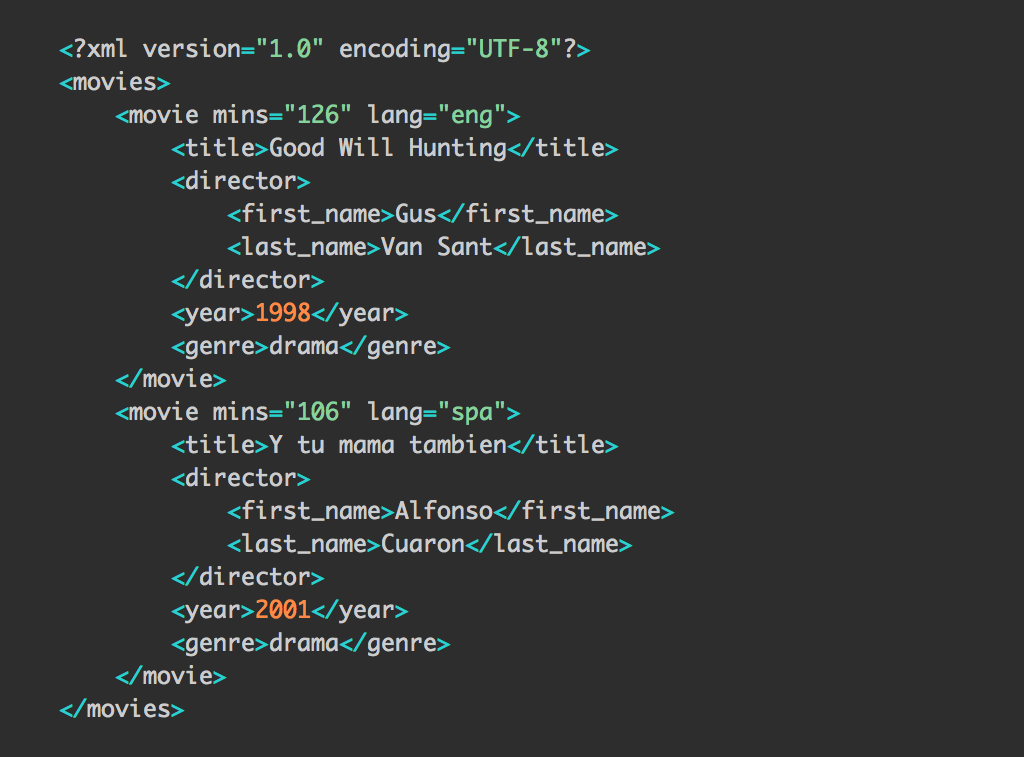
\includegraphics[width=\paperwidth]{images/xmlcover.png}
            };
        \end{tikzpicture}
     \end{frame}
}

%------------------------------------------------

\begin{frame}[fragile]
\frametitle{Readme}

\begin{block}{\scriptsize License:}
\tiny
 \begin{itemize}
  \item[] Creative Commons Attribution-NonCommercial-ShareAlike 4.0 International License \\ 
  \url{http://creativecommons.org/licenses/by-nc-sa/4.0/}{}
 \end{itemize}
\end{block}

\begin{block}{\scriptsize You are free to:}
\tiny
 \begin{itemize}
  \item[] \textcolor{darkgray}{\textbf{Share}} --- \textcolor{gray}{copy and redistribute the material}
  \item[] \textcolor{darkgray}{\textbf{Adapt}} --- \textcolor{gray}{rebuild and transform the material}
 \end{itemize}
\end{block}

\vspace{2mm}
\begin{block}{\scriptsize Under the following conditions:}
\tiny
\begin{itemize}
 \item[] \textcolor{darkgray}{\textbf{Attribution}} --- \textcolor{gray}{You must give appropriate credit, provide a link to the license, and indicate if changes were made.}
 \item[] \textcolor{darkgray}{\textbf{NonCommercial}} --- \textcolor{gray}{You may not use this work for commercial purposes.}
 \item[] \textcolor{darkgray}{\textbf{Share Alike}} --- \textcolor{gray}{If you remix, transform, or build upon this 
 work, you must distribute your contributions under the same license to this one.}
\end{itemize}
\end{block}

\end{frame}

%------------------------------------------------

\begin{frame}
\frametitle{Lectures Menu}

\begin{columns}[t]
\begin{column}{0.1\textwidth}
%--- empty space ---%
\end{column}
\begin{column}{0.8\textwidth}
 \begin{block}{Slide Decks}
  \begin{enumerate}
   \item \textcolor{lightgray}{Introduction}
   \item \textcolor{lightgray}{Reading files from the Web}
   \item \textbf{Basics of XML and HTML}
   \item \textcolor{lightgray}{Parsing XML / HTML documents}   
   \item \textcolor{lightgray}{Handling JSON data}
   \item \textcolor{lightgray}{HTTP Basics and the RCurl package}
   \item \textcolor{lightgray}{Getting data via Web Forms}
   \item \textcolor{lightgray}{Getting data via Web APIs}
  \end{enumerate}
 \end{block}
\end{column}
\begin{column}{0.1\textwidth}
%--- empty space ---%
\end{column}
\end{columns}

\end{frame}

%------------------------------------------------

\begin{frame}
 \begin{center}
  \Huge{\textcolor{mandarina}{Basics of XML \\ and HTML}}
 \end{center}
\end{frame}

%------------------------------------------------

\begin{frame}
\frametitle{Goal}

\begin{columns}[t]
\begin{column}{0.1\textwidth}
%--- empty space ---%
\end{column}
\begin{column}{0.8\textwidth}

\begin{block}{XML \& HTML}
The goal of these slides is to give you a \textbf{crash introduction to XML and HTML} so you can get a good grasp of those formats for the rest of the lectures
\end{block}

\end{column}
\begin{column}{0.1\textwidth}
%--- empty space ---%
\end{column}
\end{columns}

\end{frame}

%------------------------------------------------

\begin{frame}
\frametitle{Synopsis}

\begin{columns}[t]
\begin{column}{0.1\textwidth}
%--- empty space ---%
\end{column}
\begin{column}{0.8\textwidth}

\begin{block}{In a nutshell}
We'll cover a the following concepts:
\begin{itemize}
 \item Importance of XML and HTML
 \item Hierarchical Structure
 \item Document Object Model (DOM)
\end{itemize}
\end{block}

\end{column}
\begin{column}{0.1\textwidth}
%--- empty space ---%
\end{column}
\end{columns}

\end{frame}

%------------------------------------------------

\begin{frame}
\frametitle{Some References}

\begin{itemize}
 \item XML Files website {\scriptsize (\url{http://www.xmlfiles.com})} \\
 \low{by Jan Egil Refsnes}
 \item XML in a  Nutshell \\
 \low{by Elliotte Rusty Harold; W. Scott Means}
 \item XML Tutorial {\scriptsize (\url{http://www.w3schools.com/xml/default.asp})} \\
 \low{by w3schools}
 \item Introduction to Data Technologies \\
 \low{by Paul Murrell}
 \item XML and Web Technologies for Data Sciences with R \\
 \low{by Deb Nolan and Duncan Temple Lang}
\end{itemize}

\end{frame}

%------------------------------------------------

\begin{frame}
\frametitle{XML and HTML}

\begin{block}{Why you should care about XML and HTML?}
\begin{itemize}
  \item Large amounts of data and information are stored, shared and distributed using HTML and XML-dialects
  \item They are widely adopted and used in many applications
  \item Working with data from the Web means dealing with HTML
 \end{itemize}
\end{block}

\end{frame}


%------------------------------------------------

\begin{frame}
 \begin{center}
  {\Huge \textcolor{mandarina}{XML}} \\
  \bigskip
  {\Large \textcolor{mandarina}{eXtensible Markup Language}}
 \end{center}
\end{frame}

%------------------------------------------------

{ % all template changes are local to this group.
    \setbeamertemplate{navigation symbols}{}
    \begin{frame}[plain]
        \begin{tikzpicture}[remember picture,overlay]
            \node[at=(current page.center)] {
                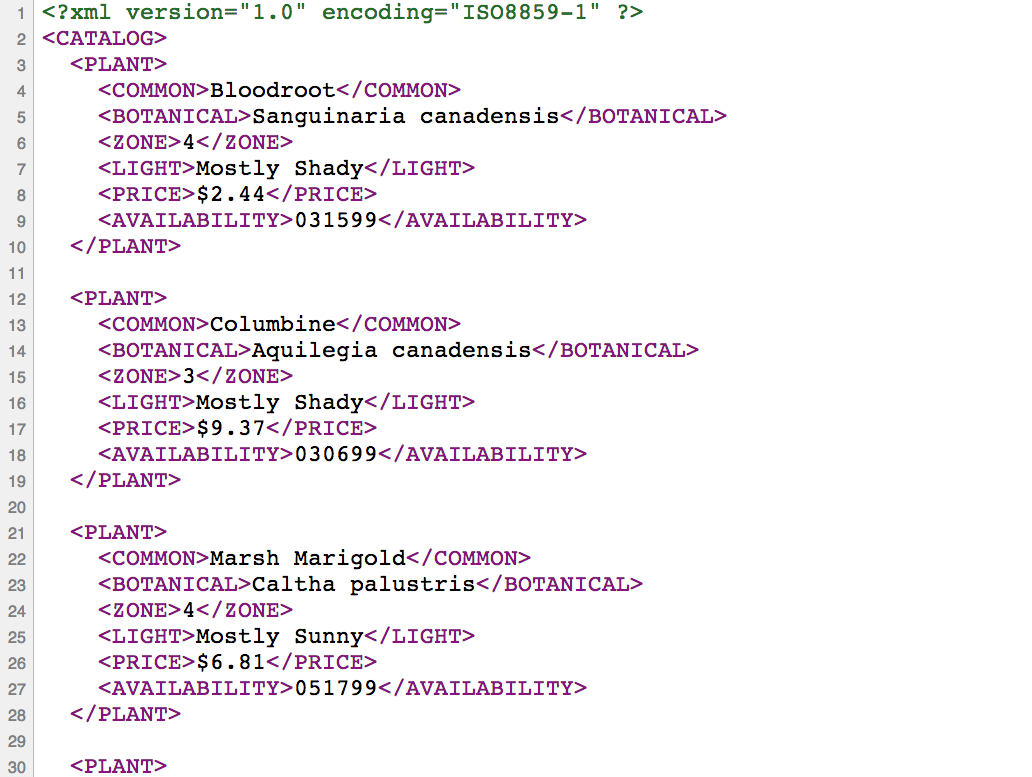
\includegraphics[width=\paperwidth]{images/xml_plants_catalog.png}
            };
        \end{tikzpicture}
     \end{frame}
}

%------------------------------------------------

\begin{frame}
\frametitle{Some Definitions}

\begin{quotation}
``XML is a markup language that defines a set of rules for encoding documents in a format that is both human-readable and machine-readable''
\end{quotation}

{\footnotesize 
\hspace{8mm} \url{http://en.wikipedia.org/wiki/XML}
}

\bigskip
\begin{quotation}
``XML is a data description language used for describing data''
\end{quotation}

{\footnotesize 
\hspace{8mm} \high{Paul Murrell} \\
\hspace{8mm} \low{Introduction to Data Technologies}
}

\end{frame}

%------------------------------------------------

\begin{frame}
\frametitle{Some Definitions}

\begin{quotation}
``XML is a very general structure with which we can define any number of new formats to represent arbitrary data''
\end{quotation}

\begin{quotation}
``XML is a standard for the semantic, hierarchical representation of data''
\end{quotation}

{\footnotesize 
\hspace{8mm} \high{Deb Nolan \& Duncan Temple Lang} \\
\hspace{8mm} \low{XML and Web Technologies for Data Sciences with R}
}

\end{frame}

%------------------------------------------------

\begin{frame}
\frametitle{About XML}

\begin{columns}[t]
\begin{column}{0.1\textwidth}
%--- empty space ---%
\end{column}
\begin{column}{0.8\textwidth}
 
\begin{block}{XML}
XML stands for \textbf{eXtensible Markup Language}
\end{block}

\begin{block}{Broadly speaking ...}
XML provides a flexible framework to create formats for describing and representing data
\end{block}

\end{column}
\begin{column}{0.1\textwidth}
%--- empty space ---%
\end{column}
\end{columns}

\end{frame}

%------------------------------------------------

\begin{frame}
\frametitle{Markups}

\begin{block}{Markup}
A \textbf{markup} is a sequence of characters or other symbols inserted at certain places in a document to indicate either: 
\begin{itemize}
 \item how the content should be displayed when printed or in screen
 \item describe the document's structure
\end{itemize}
\end{block}

\begin{block}{Markup Language}
A markup language is a system for \textbf{annotating} (i.e. \textit{marking}) a document in a way that the content is distinguished from its representation \low{(eg LaTeX, PostScript, HTML, SVG)}
\end{block}

\end{frame}

%------------------------------------------------

\begin{frame}[fragile]
\frametitle{Markups}

\begin{block}{XML Markups}
In XML (as well as in HTML) the marks (aka \textit{tags}) are defined using angle brackets: {\Huge \highcode{<>}}
\end{block}

\bigskip

\code{ \high{<mark>}Text marked with special tag\high{</mark>} }

\end{frame}

%------------------------------------------------

\begin{frame}[fragile]
\frametitle{Extensible}

\begin{block}{Extensible?}
The concept of \textit{extensibility} means that we can define our own marks, the order in which they occur, and how they should be processed. For example:
 \begin{itemize}
  \item \highcode{<my\_mark>}
  \item \highcode{<awesome>}
  \item \highcode{<boring>}
  \item \highcode{<pathetic>}
 \end{itemize}
\end{block}

\end{frame}

%------------------------------------------------

\begin{frame}
\frametitle{About XML}

\begin{block}{XML is NOT}
\begin{itemize}
 \item a programming language
 \item a network transfer protocol
 \item a database
\end{itemize}
\end{block}

\begin{block}{XML is}
\begin{itemize}
 \item more than a markup language
 \item a generic language that provides structure and syntax for representing any type of information
 \item a meta-language: it allows us to create or define other languages
\end{itemize}
\end{block}

\end{frame}

%------------------------------------------------

\begin{frame}
\frametitle{XML Applications}

\begin{block}{Some XML dialects}
\begin{itemize}
 \item \textbf{KML} (\textit{Keyhole Markup Language}) for describing geo-spatial information used in Google Earth, Google Maps, Google Sky
 \item \textbf{SVG} (\textit{Scalable Vector Graphics}) for visual graphical displays of two-dimensional graphics with support for interactivity and animation
 \item \textbf{PMML} (\textit{Predictive Model Markup Language}) for describing and exchanging models produced by data mining and machine learning algorithms
\end{itemize}
\end{block}

\end{frame}


%------------------------------------------------

\begin{frame}
\frametitle{XML Applications (con't)}

\begin{block}{Some XML dialects}
\begin{itemize}
 \item \textbf{RSS} (\textit{Rich Site Summary}) feeds for publishing blog entries
 \item \textbf{SDMX} (\textit{Statistical Data and Metadata Exchange}) for organizing and exchanging statistical information
 \item \textbf{GML} (\textit{Geography Markup Language}) for representing geographical features
 \item \textbf{SBML} (\textit{Systems Biology Markup Language}) for describing biological systems
\end{itemize}
\end{block}

\end{frame}

%------------------------------------------------

\begin{frame}
 \begin{center}
  \Huge{\textcolor{mandarina}{Minimalist Example}}
 \end{center}
\end{frame}

%------------------------------------------------

{ % all template changes are local to this group.
    \setbeamertemplate{navigation symbols}{}
    \begin{frame}[plain]
        \begin{tikzpicture}[remember picture,overlay]
            \node[at=(current page.center)] {
                
\includegraphics[width=\paperwidth]{images/goodwillhunting.jpg}
            };
        \end{tikzpicture}
     \end{frame}
}

%------------------------------------------------

\begin{frame}[fragile]
\frametitle{XML Example}

\begin{block}{Ultra Simple XML}
\begin{verbatim}
<movie>
  Good Will Hunting
</movie>
\end{verbatim}
\end{block}

\bigskip

\begin{itemize}
 \item one single element {\textit{movie}}
 \item start-tag: \highcode{<movie>}
 \item end-tag: \highcode{</movie>}
 \item content: \highcode{Good Will Hunting}
\end{itemize}

\end{frame}

%------------------------------------------------

\begin{frame}[fragile]
\frametitle{XML Example}

\begin{block}{Ultra Simple XML}
\begin{verbatim}
<movie mins="126" lang="en">
  Good Will Hunting
</movie>
\end{verbatim}
\end{block}

\bigskip

\begin{itemize}
 \item xml elements can have \textbf{attributes}
 \item attributes: \highcode{mins} \low{(minutes)} and \highcode{lang} \low{(language)}
 \item attributes are \textit{attached} to the element's start tag
 \item attribute values \textbf{must be quoted!}
\end{itemize}

\end{frame}

%------------------------------------------------

\begin{frame}[fragile]
\frametitle{XML Example}

\begin{block}{Minimalist XML}
\begin{verbatim}
<movie mins="126" lang="en">
  <title>Good Will Hunting</title>
  <director>Gus Van Sant</director>
  <year>1998</year>
  <genre>drama</genre>
</movie>
\end{verbatim}
\end{block}

\bigskip

\begin{itemize}
 \item an xml element may contain other elements
 \item \textit{movie} contains several elements: \textit{title, director, year, genre}
\end{itemize}

\end{frame}

%------------------------------------------------

\begin{frame}[fragile]
\frametitle{XML Example}

\begin{block}{Simple XML}
\begin{verbatim}
<movie mins="126" lang="en">
  <title>Good Will Hunting</title>
  <director>
    <first_name>Gus</first_name>
    <last_name>Van Sant</last_name>
  </director>
  <year>1998</year>
  <genre>drama</genre>
</movie>
\end{verbatim}
\end{block}

\bigskip

\begin{itemize}
 \item Now \textit{director} has two child elements: \textit{first\_name} and \textit{last\_name}
\end{itemize}

\end{frame}

%------------------------------------------------

\begin{frame}[fragile]
\frametitle{XML Hierarchy Structure}

\begin{block}{Conceptual XML}
\begin{verbatim}
<Root>
  <child_1>...</child_1>
  <child_2>...</child_2>
    <subchild>...</subchild>
  <child_3>...</child_3>
</Root>
\end{verbatim}
\end{block}

\bigskip

\begin{itemize}
 \item An XML document can be represented with a \textbf{tree structure}
 \item An XML document must have \textbf{one single Root} element
 \item The \code{Root} may contain \code{child} elements
 \item A \code{child} element may contain \code{subchild} elements
\end{itemize}

\end{frame}

%------------------------------------------------

\begin{frame}
\frametitle{XML Tree Structure}

\begin{center}
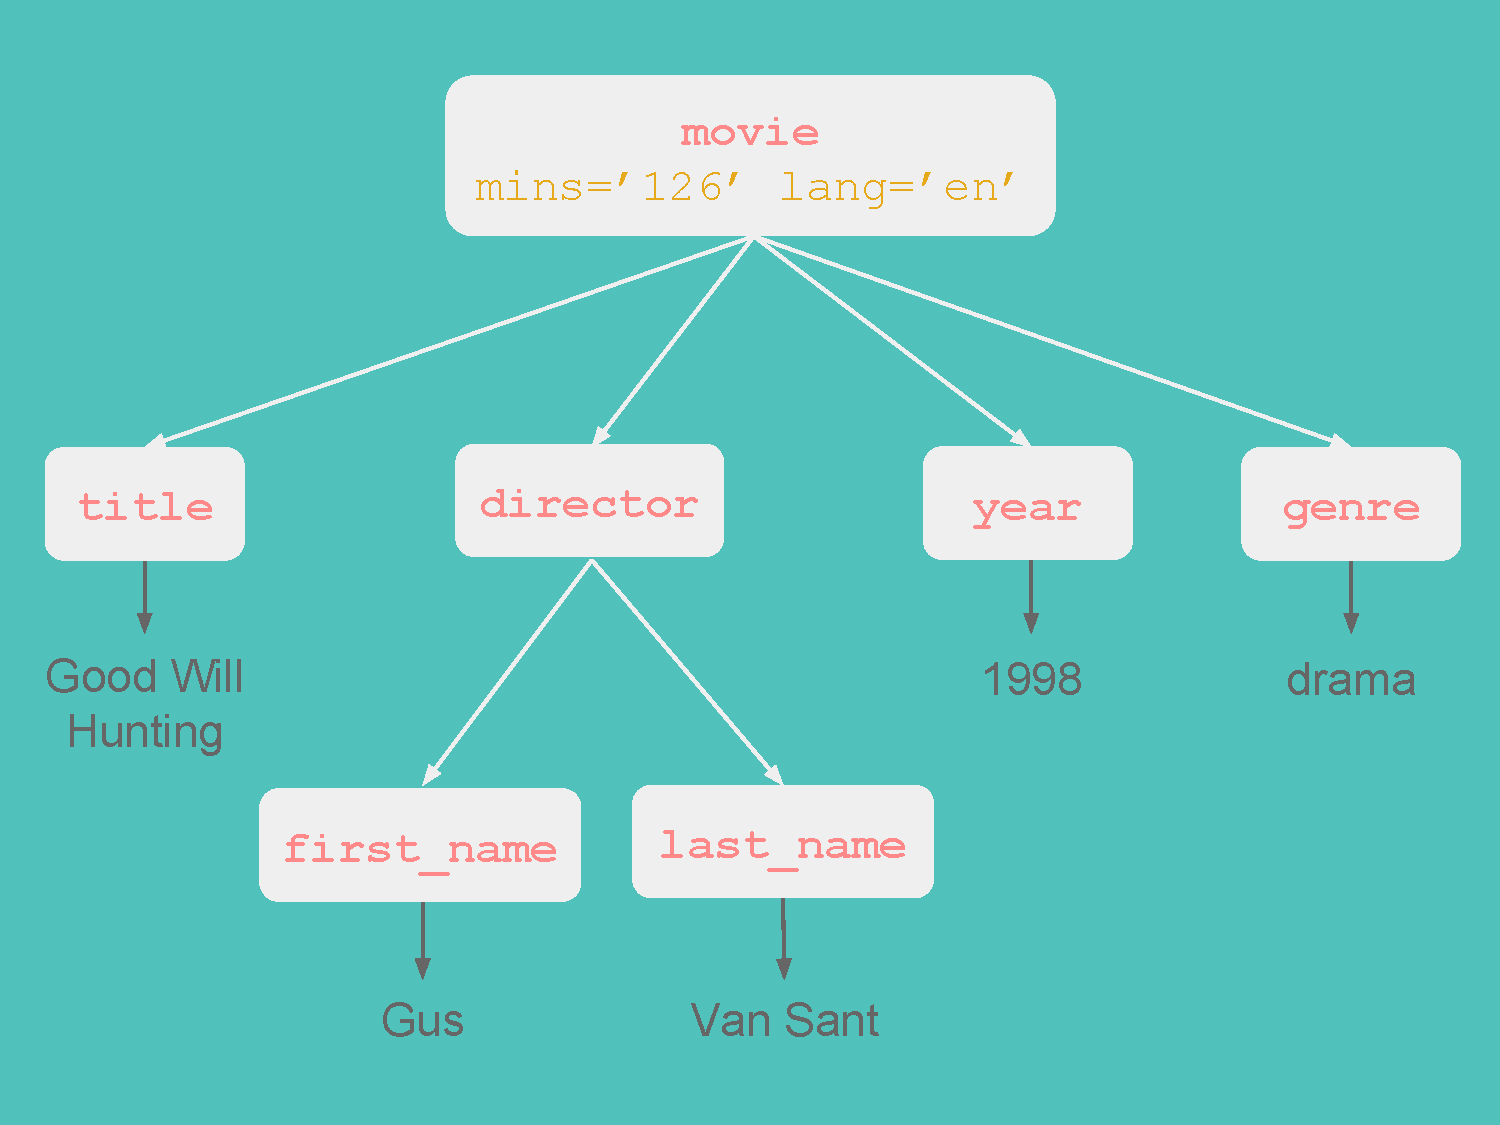
\includegraphics[width=9cm]{images/xml_movie_tree1.pdf}
\end{center}

\end{frame}

%------------------------------------------------

\begin{frame}
\frametitle{XML Tree Structure (con't)}

\begin{center}
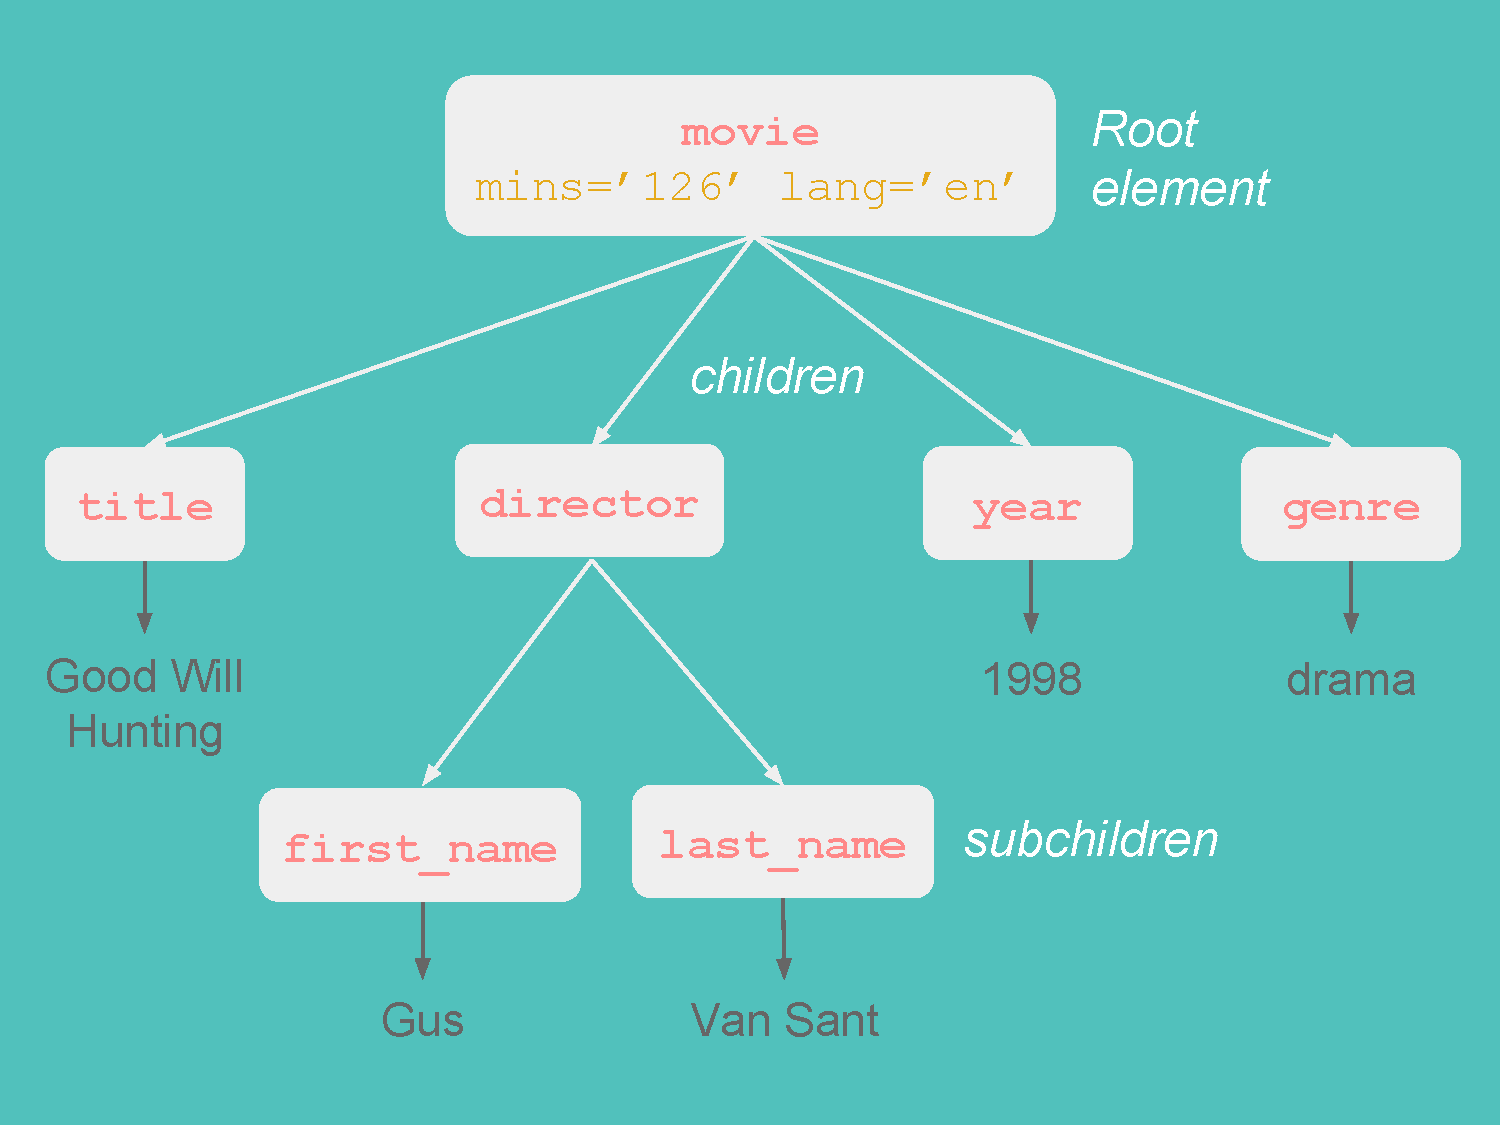
\includegraphics[width=9cm]{images/xml_movie_tree2.pdf}
\end{center}

\end{frame}

%------------------------------------------------

\begin{frame}
\frametitle{Well-Formedness}

\begin{block}{Well-formed XML}
We say that an XML document is \textbf{well-formed} when it obeys the basic syntax rules of XML. Some of those rules are:
\begin{itemize}
 \item one root element containing the rest of elements
 \item properly nested elements
 \item self-closing tags
 \item attributes appear in start-tags of elements
 \item attribute values must be quoted
 \item element names and attribute names are case sensitive
\end{itemize}
\end{block}

\end{frame}

%------------------------------------------------

\begin{frame}
\frametitle{Well-Formedness}

\begin{block}{Importance of Well-formed XML}
Not well-formed XML documents produce potentially fatal errors or warnings when parsed.

\bigskip
Documents may be well-formed but not valid. Well-formed just guarantees that the document meets the basic XML structure, not that the content is valid.
\end{block}

\end{frame}

%------------------------------------------------

\begin{frame}
 \begin{center}
  \Huge{\textcolor{mandarina}{Additional XML Elements}}
 \end{center}
\end{frame}

%------------------------------------------------

\begin{frame}[fragile]
\frametitle{Some Additional Elements}

\begin{block}{Example with extra elemets}
{ \small
\begin{verbatim}
<?xml version="1.0"? encoding="UTF-8" ?>
<![CDATA[ a > 5 & b < 10 ]]>
<?GS print(format = TRUE)>
<!DOCTYPE Movie>
<!-- This is a commet -->
<movie mins="126" lang="en">
  <title>Good Will Hunting</title>
  <director>
    <first_name>Gus</first_name>
    <last_name>Van Sant</last_name>
  </director>
  <year>1998</year>
  <genre>drama</genre>
</movie>
\end{verbatim}
}
\end{block}

\end{frame}

%------------------------------------------------

\begin{frame}
\frametitle{Additional Elements}

\begin{center}
\textcolor{turquoise}{Additional (optional) XML elements}

\bigskip
\begin{tabular}{l l}
  \hline
  Markup & Description \\
  \hline
  \code{<?xml >} & XML Declaration \\
  & \low{identifies content as an XML document} \\
  \code{<?PI >} & Processing Instruction \\
  & \low{processing instructions passed to application \code{PI}} \\
  \code{<!DOCTYPE >} & Document-type Declaration \\
  & \low{defines the structure of an XML document} \\
  \code{<![CDATA[ ]]>} & CDATA Character Data \\
  & \low{anything inside a CDATA is ignored by the parser} \\
  \code{<!--  -->} & Comment \\
  & \low{for writing comments} \\
  \hline
 \end{tabular}
\end{center}

\end{frame}

%------------------------------------------------

\begin{frame}
\frametitle{DTD}

\begin{block}{Document-Type Declaration}
The Document-type Declaration identifies the \textbf{type} of the document. The \textit{type} indicates the structure of a \textbf{valid} document: 

\begin{itemize}
 \item what elements are allowed to be present
 \item how elements can be combined
 \item how elements must be ordered
\end{itemize}
\end{block}

Basically, the DTD specifies what the format allows to do.
\end{frame}

%------------------------------------------------

\begin{frame}
 \begin{center}
  \Huge{\textcolor{mandarina}{Wrapping Up}}
 \end{center}
\end{frame}

%------------------------------------------------

\begin{frame}
\frametitle{About XML}

\begin{block}{About XML}
\begin{itemize}
 \item designed to store and transfer data
 \item designed to be self-descriptive
 \item tags are not predefined and can be extended
\end{itemize}
\end{block}

\end{frame}

%------------------------------------------------

\begin{frame}
\frametitle{Characteristics of XML}

\begin{block}{XML is}
\begin{itemize}
 \item a generic language that provides structure and syntax for many markup dialects
 \item is a syntax or format for defining markup languages
 \item a standard for the semantic, hierarchical representation of data
 \item provides a general approach for representing all types of information  dialects
\end{itemize}
\end{block}

\end{frame}

%------------------------------------------------

\begin{frame}[fragile]
\frametitle{XML document example}

\begin{block}{Simple XML}
\begin{verbatim}
<?xml version="1.0"?>
<!DOCTYPE movies>
<movie mins="126" lang="en">
  <!-- this is a comment -->
  <title>Good Will Hunting</title>
  <director>
    <first_name>Gus</first_name>
    <last_name>Van Sant</last_name>
  </director>
  <year>1998</year>
  <genre>drama</genre>
</movie>
\end{verbatim}
\end{block}

\end{frame}

%------------------------------------------------

\begin{frame}
\frametitle{XML Tree Structure}

\begin{block}{Each Node can have:}
\begin{itemize}
 \item a Name
 \item any number of attributes
 \item optional content
 \item other nested elements
\end{itemize}
\end{block}

\begin{block}{Traversing the tree}
There's a \textbf{unique} path from the root node to any given node 
\end{block}

\end{frame}

%------------------------------------------------

\end{document}
